\chapter{Leçon 25: Transportmëttelen}

Dës Lektioun beschäftegt sech mat de verschiddenen Transportmëttelen wéi Autoen, Zich, de Vëlo an de Fliger. Mir léieren och iwwer e Vëlosaccident, de Gebrauch vum Verb \textbf{kippen} an d'Reese mat Containerschëffer. \textit{Cette leçon traite des différents moyens de transport tels que les voitures, les trains, le vélo et l'avion. Nous apprenons également sur un accident de vélo, l'utilisation du verbe \textbf{kippen} et les voyages en porte-conteneurs. / This lesson deals with the different means of transport such as cars, trains, the bicycle, and the airplane. We also learn about a bicycle accident, the use of the verb \textbf{kippen}, and traveling on container ships.}

\vspace{1em}

\section[Autoen an hir Beschreiwungen / Voitures / Cars]{Autoen an hir Beschreiwungen \\/ Voitures et leurs descriptions \\/ Cars and their descriptions}

Hei sinn e puer praktesch Beispiller fir Autoen ze beschreiwen, inspiréiert vun eisen Notizen: \\
\textit{Voici quelques exemples pratiques pour décrire des voitures, inspirés de nos notes : / Here are some practical examples for describing cars, inspired by our notes:}

\begin{itemize}
    \item \textbf{Ech wéilt gär en elektresche Kia kafen.} \\
    \textit{Je voudrais acheter une Kia électrique. / I would like to buy an electric Kia.}
    
    \item \textbf{Hatt huet e grousse BMW, dee fofzéng Joer an en halleft al ass. Et ass en Diesel an hatt huet keng grouss Problemer, awer d'Revisioun gëtt net bei BMW gemaach.} \\
    \textit{Elle a une grande BMW qui a quinze ans et demi. C'est une diesel et elle n'a pas de grands problèmes, mais la révision n'est pas faite chez BMW. / She has a big BMW that is fifteen and a half years old. It is a diesel and has no big problems, but the servicing is not done at BMW.}
    
    \item \textbf{Mäin Dramauto war e giele Porsche fir fofzegdausend Euro op Facebook. Mee ech hu keen Dramauto méi.} \\
    \textit{Ma voiture de rêve était une Porsche jaune à 50 000 euros sur Facebook. Mais je n'ai plus de voiture de rêve. / My dream car was a yellow Porsche for 50,000 euros on Facebook. But I don't have a dream car anymore.}
    
    \item \textbf{Hien huet e schwaarze BMW, deen net nei ass. En ass zimmlech gemittlech, vu 2019, e Benziner mat enger Automatik-Boîte.} \\
    \textit{Il a une BMW noire qui n'est pas neuve. Elle est assez confortable, de 2019, une essence avec boîte automatique. / He has a black BMW that is not new. It is quite comfortable, from 2019, a petrol engine with an automatic gearbox.}
    
    \item \textbf{Ech hu keen Auto méi. Ech wéilt gär e BYD Atto 2 hunn, am beschten a wäisser Faarf.} \\
    \textit{Je n'ai plus de voiture. Je voudrais avoir une BYD Atto 2, de préférence de couleur blanche. / I don't have a car anymore. I would like to have a BYD Atto 2, preferably in white.}
    
    \item \textbf{Ech hunn en Audi A3 Sportback vun 2010. D'Reparatur ass deier, mee bis dräidausend Euro ass et an der Rei fir en ze flécken.} \\
    \textit{J'ai une Audi A3 Sportback de 2010. La réparation est chère, mais jusqu'à 3 000 euros, c'est acceptable pour la réparer. / I have a 2010 Audi A3 Sportback. The repair is expensive, but up to 3,000 euros, it is okay to repair it.}
    
    \item \textbf{Hie fiert e Land Rover.} \\
    \textit{Il conduit un Land Rover. / He drives a Land Rover.}
    
    \item \textbf{Am Moment weess ech net, wat fir en Auto ech soll kafen.} \\
    \textit{En ce moment, je ne sais pas quelle voiture je devrais acheter. / At the moment, I don't know what car I should buy.}
    
    \item \textbf{Kann een de Récksëtz no vir kippen oder leeën, fir méi Plaz an der Mall ze kréien?} \\
    \textit{Peut-on basculer ou rabattre le siège arrière vers l'avant pour avoir plus de place dans le coffre ? / Can one tilt or lay the back seat forward to get more space in the trunk?}
    
    \item \textbf{Eeler Leit hu méi Angscht wéi déi Jonk wärend dem Fueren.} \\
    \textit{Les personnes âgées ont plus peur que les jeunes en conduisant. / Older people are more afraid than young people while driving.}
    
    \item \textbf{Wann ech am Auto liesen, gëtt et mir schwindeleg (oder dronken am Kapp).} \\
    \textit{Quand je lis en voiture, j'ai le mal des transports (vertiges). / When I read in the car, I get dizzy / motion sick (or lightheaded).}
    
    \item \textbf{Ech kann haut net fueren, ech sinn dronken. Mir mussen en Taxi huelen.} \\
    \textit{Je ne peux pas conduire aujourd'hui, je suis ivre. Nous devons prendre un taxi. / I cannot drive today, I am drunk. We must take a taxi.}
    
    \item \textbf{Wann ee mat engem Fliger iwwer de Grand Canyon flitt, gesäit e Mënsch wéi eng Méck aus.} \\
    \textit{Quand on survole le Grand Canyon en avion, un être humain ressemble à une mouche. / When you fly over the Grand Canyon in a plane, a human looks like a fly.}
\end{itemize}

\vspace{1cm}

\section[D'Verben an hire Gebrauch / Verbes / Verbs]{D'Verben an hire Gebrauch \\/ Les verbes et leur utilisation \\/ Verbs and their usage}

An dëser Lektioun hu mir e puer wichteg Verben begéint. Hei sinn hir Konjugatiounen an hir verschidde Bedeitungen: \\
\textit{Dans cette leçon, nous avons rencontré plusieurs verbes importants. Voici leurs conjugaisons et leurs différentes significations : / In this lesson, we encountered several important verbs. Here are their conjugations and different meanings:}

\subsection*{1. Kippen}
D'Verb \textbf{kippen} huet verschidde Bedeitungen am Lëtzebuergeschen:
\begin{itemize}
    \item \textbf{Basculer / rabattre / coucher} (to tilt / fold down / lay flat): \textit{de Récksëtz no vir kippen oder leeën, fir méi Plaz an der Mall ze kréien.} \\
    $\rightarrow$ French: \textit{basculer ou rabattre le siège arrière vers l'avant pour avoir plus de place dans le coffre.} \\
    $\rightarrow$ English: \textit{to tilt or fold/lay the back seat forward to get more space in the trunk.}
    
    \item \textbf{Se renverser / tomber} (to tip over / fall): \textit{D'Fläsch ass gekippt.} / \textit{Ëmkippen} (ëmgangssproochlech: ze falen / stierzen): \textit{Ech sinn ëmgekippt.} \\
    $\rightarrow$ French: \textit{La bouteille a basculé. / Je suis tombé (de vélo).} \\
    $\rightarrow$ English: \textit{The bottle tipped over. / I tipped over (fell off the bicycle).}
    
    \item \textbf{Décharger / vider} (to dump / pour out): \textit{Steng aus der Karet kippen.} \\
    $\rightarrow$ French: \textit{décharger des pierres d'une brouette.} \\
    $\rightarrow$ English: \textit{to dump stones from a wheelbarrow.}
    
    \item \textbf{Boire d'un trait} (colloquial: to down / chug a drink): \textit{En Humpen Béier erofkippen.} \\
    $\rightarrow$ French: \textit{s'enfiler une chope de bière (boire d'un trait).} \\
    $\rightarrow$ English: \textit{to down a pint of beer.}
\end{itemize}

\begin{tabular}{ll c l l}
    \toprule
    \textbf{Pronom} & \textbf{Lëtzebuergesch} & \textbf{} & \textbf{Français} & \textbf{English} \\
    \midrule
    ech & kippen & $\rightarrow$ & Je bascule & I tilt / tip \\
    du & kipps & $\rightarrow$ & Tu bascules & You tilt / tip \\
    hien / hatt / et & kippt & $\rightarrow$ & Il / Elle bascule & He / She tilts / tips \\
    \midrule
    mir & kippen & $\rightarrow$ & Nous basculons & We tilt / tip \\
    dir & kippt & $\rightarrow$ & Vous basculez & You tilt / tip \\
    si & kippen & $\rightarrow$ & Ils basculent & They tilt / tip \\
    \bottomrule
\end{tabular}
\\[0.5em]
\textbf{Imperativ:} Kipp! Kippt! (Bascule ! Basculez ! / Tilt!) \\
\textbf{Passé Composé:} Forméiert mat \textit{hunn} + \textbf{gekippt} (oder \textit{sinn} + \textbf{ëmgekippt} fir d'Aktioun vum Falen).

\subsection*{2. Strampelen}
D'Verb \textbf{strampelen} ass en ëmgangssproochlecht (colloquial) Verb fir haart ze pedalen oder d'Féiss kräfteg ze bewegen:
\begin{itemize}
    \item \textbf{Pédaler fort} (to pedal hard / struggle): \textit{Am Bierg hu mir musse strampelen.} \\
    $\rightarrow$ French: \textit{Dans la montée, nous avons dû pédaler fort.} \\
    $\rightarrow$ English: \textit{On the climb, we had to pedal hard.}
    
    \item \textbf{Gigoter} (to kick legs / struggle): \textit{De Puppelche strampelt wëll.} \\
    $\rightarrow$ French: \textit{Le bébé gigote vigoureusement.} \\
    $\rightarrow$ English: \textit{The baby kicks its legs wildly.}
\end{itemize}

\begin{tabular}{ll c l l}
    \toprule
    \textbf{Pronom} & \textbf{Lëtzebuergesch} & \textbf{} & \textbf{Français} & \textbf{English} \\
    \midrule
    ech & strampelen & $\rightarrow$ & Je pédale fort / gigote & I pedal hard / kick \\
    du & strampels & $\rightarrow$ & Tu pédales fort & You pedal hard \\
    hien / hatt / et & strampelt & $\rightarrow$ & Il / Elle pédale fort & He / She pedals hard \\
    \midrule
    mir & strampelen & $\rightarrow$ & Nous pédalons fort & We pedal hard \\
    dir & strampelt & $\rightarrow$ & Vous pédalez fort & You pedal hard \\
    si & strampelen & $\rightarrow$ & Ils pédalent fort & They pedal hard \\
    \bottomrule
\end{tabular}
\\[0.5em]
\textbf{Passé Composé:} Forméiert mat \textit{hunn} + \textbf{gestrampelt}.

\subsection*{3. Ophänken}
D'Verb \textbf{ophänken} ka folgend Bedeitunge hunn:
\begin{itemize}
    \item \textbf{Suspendre / accrocher} (to hang up clothes/pictures): \textit{Biller un d'Mauer ophänken.} \\
    $\rightarrow$ French: \textit{accrocher des tableaux au mur.} \\
    $\rightarrow$ English: \textit{to hang pictures on the wall.}
    
    \item \textbf{Raccrocher le téléphone} (to hang up the phone): \textit{Ech hunn den Telefon opgehaangen.} \\
    $\rightarrow$ French: \textit{J'ai raccroché le téléphone.} \\
    $\rightarrow$ English: \textit{I hung up the phone.}
    
    \item \textbf{Eppes un den Nol hänken} (idiom: abandonner/arrêter une activité, « suspendre au clou » / to hang something on the nail, i.e., to give up on or retire from something): \textit{Ech hu mäin Dramauto un den Nol gehaangen.} \\
    $\rightarrow$ French: \textit{J'ai fait une croix sur mon projet de voiture de rêve.} \\
    $\rightarrow$ English: \textit{I gave up on my dream car (hung it on the nail).}
\end{itemize}

\begin{tabular}{ll c l l}
    \toprule
    \textbf{Pronom} & \textbf{Lëtzebuergesch} & \textbf{} & \textbf{Français} & \textbf{English} \\
    \midrule
    ech & hänken op & $\rightarrow$ & J'accroche / raccroche & I hang up \\
    du & hänks op & $\rightarrow$ & Tu accroches & You hang up \\
    hien / hatt / et & hänkt op & $\rightarrow$ & Il / Elle accroche & He / She hangs up \\
    \midrule
    mir & hänken op & $\rightarrow$ & Nous accrochons & We hang up \\
    dir & hänkt op & $\rightarrow$ & Vous accrochez & You hang up \\
    si & hänken op & $\rightarrow$ & Ils accrochent & They hang up \\
    \bottomrule
\end{tabular}
\\[0.5em]
\textbf{Passé Composé:} Forméiert mat \textit{hunn} + \textbf{opgehaangen}.

\subsection*{4. Richen}
D'Verb \textbf{richen} (sentir / to smell) gehéiert zu de wichtege Verben fir Sënner:

\begin{tabular}{ll c l l}
    \toprule
    \textbf{Pronom} & \textbf{Lëtzebuergesch} & \textbf{} & \textbf{Français} & \textbf{English} \\
    \midrule
    ech & richen & $\rightarrow$ & Je sens & I smell \\
    du & richs & $\rightarrow$ & Tu sens & You smell \\
    hien / hatt / et & richt & $\rightarrow$ & Il / Elle sent & He / She smells \\
    \midrule
    mir & richen & $\rightarrow$ & Nous sentons & We smell \\
    dir & richt & $\rightarrow$ & Vous sentez & You smell \\
    si & richen & $\rightarrow$ & Ils sentent & They smell \\
    \bottomrule
\end{tabular}
\\[0.5em]
\textbf{Beispill:} \textit{Et richt no Mazut.} (Ça sent le mazout. / It smells of fuel oil.) \\
\textbf{Passé Composé:} Forméiert mat \textit{hunn} + \textbf{geroch}.

\subsection*{5. Fléien}
D'Verb \textbf{fléien} (voler / to fly) ass en onreegelméissegt Verb:

\begin{tabular}{ll c l l}
    \toprule
    \textbf{Pronom} & \textbf{Lëtzebuergesch} & \textbf{} & \textbf{Français} & \textbf{English} \\
    \midrule
    ech & fléien & $\rightarrow$ & Je vole & I fly \\
    du & flitts & $\rightarrow$ & Tu voles & You fly \\
    hien / hatt / et & flitt & $\rightarrow$ & Il / Elle vole & He / She flies \\
    \midrule
    mir & fléien & $\rightarrow$ & Nous volons & We fly \\
    dir & flitt & $\rightarrow$ & Vous volez & You fly \\
    si & fléien & $\rightarrow$ & Ils volent & They fly \\
    \bottomrule
\end{tabular}
\\[0.5em]
\textbf{Passé Composé:} Forméiert mat \textit{sinn} + \textbf{geflunn} (fir d'Aktioun vun der Rees).

\subsection*{6. Flécken}
D'Verb \textbf{flécken} (réparer, raccommoder / to repair, fix, mend):

\begin{tabular}{ll c l l}
    \toprule
    \textbf{Pronom} & \textbf{Lëtzebuergesch} & \textbf{} & \textbf{Français} & \textbf{English} \\
    \midrule
    ech & flécken & $\rightarrow$ & Je répare & I repair \\
    du & flécks & $\rightarrow$ & Tu répares & You repair \\
    hien / hatt / et & fléckt & $\rightarrow$ & Il / Elle répare & He / She repairs \\
    \midrule
    mir & flécken & $\rightarrow$ & Nous réparons & We repair \\
    dir & fléckt & $\rightarrow$ & Vous réparez & You repair \\
    si & flécken & $\rightarrow$ & Ils réparent & They repair \\
    \bottomrule
\end{tabular}
\\[0.5em]
\textbf{Passé Composé:} Forméiert mat \textit{hunn} + \textbf{gefléckt}.

\vspace{1cm}

\section[De Vëlosaccident / L'accident de vélo / The bicycle accident]{De Vëlosaccident \\/ L'accident de vélo \\/ The bicycle accident}

\noindent\textbf{1. Ech fuere gär Vëlo, a mäi Jong huet och e Vëlo. En ass orange, awer net elektresch.}\\
\textit{Ech fuere gär} (J'aime faire / I like to ride) \textit{Vëlo} (du vélo / a bicycle), \textit{a mäi Jong} (et mon fils / and my son) \textit{huet och} (a aussi / also has) \textit{e Vëlo} (un vélo / a bicycle). \textit{En ass orange} (Il est orange / It is orange), \textit{awer net elektresch} (mais pas électrique / but not electric).\\
$\rightarrow$ Français : \textit{J'aime faire du vélo, et mon fils a aussi un vélo. Il est orange, mais il n'est pas électrique.}\\
$\rightarrow$ English : \textit{I like to ride a bicycle, and my son also has a bicycle. It is orange, but not electric.}\\[0.5em]

\noindent\textbf{2. Mir fueren dacks zesumme mam Vëlo, awer hie fiert och gär en elektresche Scooter (Trottinett).}\\
\textit{Mir fueren dacks} (Nous roulons souvent / We often ride) \textit{zesumme} (ensemble / together) \textit{mam Vëlo} (à vélo / by bicycle), \textit{awer hie fiert och gär} (mais il aime aussi rouler / but he also likes to ride) \textit{en elektresche Scooter} (une trottinette électrique / an electric scooter).\\
$\rightarrow$ Français : \textit{Nous faisons souvent du vélo ensemble, mais il aime aussi faire de la trottinette électrique.}\\
$\rightarrow$ English : \textit{We often ride bicycles together, but he also likes to ride an electric scooter.}\\[0.5em]

\noindent\textbf{3. Eng Kéier si mir mam Jong op de Séi gefuer. Dat war déi eenzeg Kéier, wou ech ouni Helm war.}\\
\textit{Eng Kéier} (Une fois / One time) \textit{si mir gefuer} (sommes-nous allés / we rode) \textit{mam Jong} (avec le garçon/fils / with the boy/son) \textit{op de Séi} (au lac / to the lake). \textit{Dat war} (C'était / That was) \textit{déi eenzeg Kéier} (la seule fois / the only time), \textit{wou ech ouni Helm war} (où j'étais sans casque / where I was without a helmet).\\
$\rightarrow$ Français : \textit{Une fois, je suis allée au lac avec mon fils. C'était la seule fois où je n'avais pas de casque.}\\
$\rightarrow$ English : \textit{Once, I rode to the lake with my son. That was the only time I was without a helmet.}\\[0.5em]

\noindent\textbf{4. Dunn ass eng Harespel op mäi Kapp geflunn an ech hu versicht, se mat der Hand ewechzedreiwen.}\\
\textit{Dunn ass geflunn} (Puis a volé / Then flew) \textit{eng Harespel} (une guêpe / a wasp) \textit{op mäi Kapp} (sur ma tête / onto my head), \textit{an ech hu versicht} (et j'ai essayé / and I tried) \textit{se ewechzedreiwen} (de la chasser / to drive it away) \textit{mat der Hand} (avec la main / with the hand).\\
$\rightarrow$ Français : \textit{Puis une guêpe est venue sur ma tête et j'ai essayé de la chasser avec ma main.}\\
$\rightarrow$ English : \textit{Then a wasp flew onto my head and I tried to drive it away with my hand.}\\[0.5em]

\noindent\textbf{5. Dobäi sinn ech mam Vëlo gerutscht an op der Strooss ganz béiss gefall. Aner Vëlosfuerer si just laanscht mech gefuer.}\\
\textit{Dobäi} (Ce faisant, en même temps / In doing so) \textit{sinn ech gerutscht} (j'ai glissé / I slipped) \textit{mam Vëlo} (avec le vélo / on the bicycle) \textit{an op der Strooss... gefall} (et je suis tombée sur la route / and fell on the road) \textit{ganz béiss} (très gravement / very badly). \textit{Aner Vëlosfuerer} (D'autres cyclistes / Other cyclists) \textit{si just laanscht mech gefuer} (sont juste passés à côté de moi / just rode past me).\\
$\rightarrow$ Français : \textit{Ce faisant, j'ai glissé avec le vélo et je suis tombée très lourdement sur la route. D'autres cyclistes sont juste passés à côté de moi sans s'arrêter.}\\
$\rightarrow$ English : \textit{In doing so, I slipped on the bicycle and fell very badly on the road. Other cyclists just rode past me.}\\[0.5em]

\noindent\textbf{6. Ech louch do fir ongeféier zéng Minutten an ech konnt net ootmen. Ech hat esou vill Angscht a war eleng hei zu Jonglënster.}\\
\textit{Ech louch do} (Je me tenais allongée là / I lay there) \textit{fir ongeféier} (pendant environ / for about) \textit{zéng Minutten} (dix minutes / ten minutes) \textit{an ech konnt net ootmen} (et je ne pouvais pas respirer / and I couldn't breathe). \textit{Ech hat esou vill Angscht} (J'avais tellement peur / I was so afraid) \textit{an ech war eleng} (et j'étais seule / and I was alone) \textit{hei zu Jonglënster} (ici à Junglinster / here in Junglinster).\\
$\rightarrow$ Français : \textit{Je suis restée allongée là pendant environ dix minutes sans pouvoir respirer. J'avais tellement peur et j'étais seule ici à Junglinster.}\\
$\rightarrow$ English : \textit{I lay there for about ten minutes and I couldn't breathe. I was so afraid and I was alone here in Junglinster.}\\[0.5em]

\noindent\textbf{7. Fir dem Jong keng Angscht ze maachen, hunn ech de Vëlo geholl a mir sinn op de Bus gaangen.}\\
\textit{Fir dem Jong} (Pour le garçon / To the boy) \textit{keng Angscht ze maachen} (ne pas faire peur / not to scare), \textit{hunn ech de Vëlo geholl} (j'ai pris le vélo / I took the bicycle) \textit{a mir sinn... gaangen} (et nous sommes allés / and we went) \textit{op de Bus} (au bus / to the bus).\\
$\rightarrow$ Français : \textit{Pour ne pas faire peur à mon fils, j'ai pris le vélo et nous sommes allés prendre le bus.}\\
$\rightarrow$ English : \textit{To not scare the boy, I took the bicycle and we went to the bus.}\\[0.5em]

\noindent\textbf{8. Kee Mënsch huet gehollef, de Vëlo an de Bus ze kréien. A wéi mir hu missen ausklammen, si grad zwanzeg Leit erakomm.}\\
\textit{Kee Mënsch} (Personne / Nobody) \textit{huet gehollef} (n'a aidé / helped) \textit{de Vëlo... ze kréien} (à faire entrer le vélo / to get the bicycle) \textit{an de Bus} (dans le bus / into the bus). \textit{A wéi mir hu missen} (Et quand nous avons dû / And when we had to) \textit{ausklammen} (descendre / get off), \textit{si grad} (sont juste / just then) \textit{zwanzeg Leit} (vingt personnes / twenty people) \textit{erakomm} (entrées / entered).\\
$\rightarrow$ Français : \textit{Personne n'a aidé à monter le vélo dans le bus. Et quand nous avons dû descendre, vingt personnes entraient en même temps.}\\
$\rightarrow$ English : \textit{Nobody helped to get the bicycle into the bus. And when we had to get off, twenty people were just entering.}\\[0.5em]

\noindent\textbf{9. Den aneren Dag hat ech e bloe Fleck am Gesiicht. Wéi ech d'Bak beréiert hunn, hunn ech eppes an der Nues gespuert.}\\
\textit{Den aneren Dag} (Le lendemain / The next day) \textit{hat ech} (j'avais / I had) \textit{e bloe Fleck} (un bleu / a blue spot) \textit{am Gesiicht} (sur le visage / on the face). \textit{Wéi ech... beréiert hunn} (Quand j'ai touché / When I touched) \textit{d'Bak} (la joue / the cheek), \textit{hunn ech gespuert} (j'ai ressenti / I felt) \textit{eppes} (quelque chose / something) \textit{an der Nues} (dans le nez / in the nose).\\
$\rightarrow$ Français : \textit{Le lendemain, j'avais un bleu sur le visage. Quand j'ai touché ma joue, j'ai senti quelque chose dans le nez.}\\
$\rightarrow$ English : \textit{The next day I had a bruise on my face. When I touched my cheek, I felt something in my nose.}\\[0.5em]

\noindent\textbf{10. Dat war iwwer de Weekend. De Méindeg huet den Dokter mech geschéckt fir Röntgenbilder ze maachen, an et huet sech erausgestallt, datt dräi Rëpper an och d'Augehiel gebrach waren. Dat huet zwee Joer gebraucht fir erëm ze heelen.}\\
\textit{Dat war} (C'était / That was) \textit{iwwer de Weekend} (pendant le week-end / over the weekend). \textit{De Méindeg} (Le lundi / On Monday) \textit{huet den Dokter... geschéckt} (le médecin a envoyé / the doctor sent) \textit{mech} (moi / me) \textit{fir Röntgenbilder ze maachen} (pour faire des radiographies / to take X-rays), \textit{an et huet sech erausgestallt} (et il s'est avéré / and it turned out), \textit{datt dräi Rëpper} (que trois côtes / that three ribs) \textit{an och d'Augehiel} (et aussi l'orbite / and also the eye socket) \textit{gebrach waren} (étaient cassées / were broken). \textit{Dat huet... gebraucht} (Cela a pris / That took) \textit{zwee Joer} (deux ans / two years) \textit{fir erëm ze heelen} (pour guérir à nouveau / to heal again).\\
$\rightarrow$ Français : \textit{C'était pendant le week-end. Le lundi, le médecin m'a envoyée faire des radiographies, et il s'est avéré que trois côtes ainsi que l'orbite étaient fracturées. Il a fallu deux ans pour guérir complètement.}\\
$\rightarrow$ English : \textit{That was over the weekend. On Monday, the doctor sent me to do X-rays, and it turned out that three ribs and also the eye socket were broken. It took two years to heal.}

\vspace{1cm}

\section[Reese mat engem Containerschëff / Voyage / Travel]{Reese mat engem Containerschëff \\/ Voyager sur un porte-conteneurs \\/ Traveling on a container ship}

Hei ass eng interessant Diskussioun iwwer alternativ Reesen: \\
\textit{Voici une discussion intéressante sur les voyages alternatifs : / Here is an interesting discussion about alternative travels:}

\begin{itemize}
    \item \textbf{Wousst Dir, datt een op engem Containerschëff vun Däitschland an d'USA reese kann?} \\
    \textit{Saviez-vous qu'on peut voyager sur un porte-conteneurs de l'Allemagne aux États-Unis ? / Did you know that one can travel on a container ship from Germany to the USA?}
    
    \item \textbf{D'Passagéier reesen zesumme mat der Crew. Et ginn net vill Passagéier, déi dat gläichzäiteg maache kënnen.} \\
    \textit{Les passagers voyagent avec l'équipage. Il n'y a pas beaucoup de passagers qui peuvent le faire simultanément. / The passengers travel together with the crew. There are not many passengers who can do it simultaneously.}
    
    \item \textbf{Dës Rees ass méi deier wéi e Fliger. D'Rees ka ronn eelef Deeg daueren, awer een ësst zesumme mat der Crew.} \\
    \textit{Ce voyage est plus cher qu'un vol en avion. Le voyage peut durer environ onze jours, mais on mange avec l'équipage. / This trip is more expensive than an airplane. The trip can take about eleven days, but one eats together with the crew.}
    
    \item \textbf{Wann een e bestëmmten Alter erreecht huet, brauch een e Certificat médical fir matzegoen. Well wann eppes wärend der Rees passéiert, gëtt et keen Dokter u Bord.} \\
    \textit{Lorsqu'on atteint un certain âge, on a besoin d'un certificat médical pour voyager. Car si quelque chose se produit pendant le voyage, il n'y a pas de médecin à bord. / When you reach a certain age, you need a medical certificate to travel. Because if something happens during the trip, there is no doctor on board.}
\end{itemize}

\vspace{1cm}

\section[Froen an Äntwerten fir de Sproochentest]{Froen an Äntwerten fir de Sproochentest \\/ Questions et Réponses pour l'examen de langue \\/ Questions and Answers for the language test}

Hei sinn déi typesch Froen iwwer d'Transportmëttelen an hir Äntwerten: \\
\textit{Voici les questions typiques sur les moyens de transport et leurs réponses : / Here are the typical questions about transport and their answers:}

\vspace{1em}

\noindent\textbf{1. Vu wou kommt Dir elo?}\\
\textit{D'où venez-vous maintenant ? / Where are you coming from now?}\\
\textbf{Option A:} Ech kommen elo vun der Aarbecht. \textit{(Je viens maintenant du travail. / I am coming from work now.)}\\
\textbf{Option B:} Ech kommen elo vun doheem. \textit{(Je viens maintenant de la maison. / I am coming from home now.)}\\[1em]

\noindent\textbf{2. Wéi sidd Dir haut an den INL komm? Wéi sidd Dir haut an de Sproochentest komm?}\\
\textit{Comment êtes-vous venu à l'INL aujourd'hui ? Comment êtes-vous venu à l'examen aujourd'hui ? / How did you come to the INL today? How did you come to the language test today?}\\
\textbf{Option A:} Ech si mam Bus an den INL komm, well den ëffentlechen Transport gratis ass. \textit{(Je suis venu à l'INL en bus, car les transports publics sont gratuits. / I came to the INL by bus because public transport is free.)}\\
\textbf{Option B:} Ech si mam Auto komm an ech hu mäin Auto am Parking geparkt. \textit{(Je suis venu en voiture et j'ai garé ma voiture au parking. / I came by car and I parked my car in the parking lot.)}\\[1em]

\noindent\textbf{3. Hutt Dir en Auto?}\\
\textit{Avez-vous une voiture ? / Do you have a car?}\\
\textbf{Option A:} Jo, ech hunn en elektreschen Auto vun der Mark Kia. \textit{(Oui, j'ai une voiture électrique de la marque Kia. / Yes, I have an electric car of the brand Kia.)}\\
\textbf{Option B:} Nee, ech hu keen Auto méi. Ech wéilt gär en neien Auto kafen. \textit{(Non, je n'ai plus de voiture. Je voudrais en acheter une nouvelle. / No, I don't have a car anymore. I would like to buy a new one.)}\\[1em]

\noindent\textbf{4. Hutt Dir e Führerschäin / Fürerschäin?}\\
\textit{Avez-vous un permis de conduire ? / Do you have a driver's license?}\\
\textbf{Option A:} Jo, ech hunn mäi Führerschäin scho zanter zwanzeg Joer. \textit{(Oui, j'ai mon permis de conduire depuis déjà vingt ans. / Yes, I have had my driver's license for twenty years already.)}\\
\textbf{Option B:} Jo, ech hu mäi Führerschäin a mengem Heemechtsland gemaach. \textit{(Oui, j'ai passé mon permis de conduire dans mon pays d'origine. / Yes, I got my driver's license in my home country.)}\\[1em]

\noindent\textbf{5. Wat fir Transportmëttele gëtt et zu Lëtzebuerg?}\\
\textit{Quels moyens de transport y a-t-il au Luxembourg ? / What means of transport are there in Luxembourg?}\\
\textbf{Option A:} Zu Lëtzebuerg gëtt et den Auto, de Bus, den Zuch, den Tram an de Vëlo. \textit{(Au Luxembourg, il y a la voiture, le bus, le train, le tram et le vélo. / In Luxembourg, there are the car, the bus, the train, the tram, and the bicycle.)}\\
\textbf{Option B:} Et gëtt och vill elektresch Scooter an der Stad. \textit{(Il y a aussi beaucoup de trottinettes électriques en ville. / There are also many electric scooters in the city.)}\\[1em]

\noindent\textbf{6. Wat fir Transportmëttele benotzt Dir fir schaffen ze goen?}\\
\textit{Quels moyens de transport utilisez-vous pour aller travailler ? / What means of transport do you use to go to work?}\\
\textbf{Option A:} Ech fueren normalerweis mam Auto op d'Aarbecht. \textit{(Je vais normalement au travail en voiture. / I normally drive to work by car.)}\\
\textbf{Option B:} Ech benotzen den Zuch an den Tram, well dat ganz praktesch ass. \textit{(J'utilise le train et le tram, car c'est très pratique. / I use the train and the tram because it is very practical.)}\\[1em]

\noindent\textbf{7. Fuert Dir op d’Aarbecht mam Auto? Wou parkt Dir Ären Auto?}\\
\textit{Allez-vous au travail en voiture ? Où garez-vous votre voiture ? / Do you drive to work by car? Where do you park your car?}\\
\textbf{Option A:} Jo, ech fueren mam Auto an ech parken en am Parking vun der Firma. \textit{(Oui, je vais en voiture et je la gare au parking de l'entreprise. / Yes, I drive by car and park it in the company's parking lot.)}\\
\textbf{Option B:} Nee, ech fueren net mam Auto, mee wann ech e benotzen, parken ech op engem P+R. \textit{(Non, je ne vais pas en voiture, mais quand je l'utilise, je me gare sur un P+R. / No, I don't drive to work, but when I use it, I park at a P+R.)}\\[1em]

\noindent\textbf{8. Wat fir en Transport benotzt Dir am meeschten?}\\
\textit{Quel transport utilisez-vous le plus ? / Which transport do you use the most?}\\
\textbf{Option A:} Ech benotzen de Bus am meeschten, well e gratis ass a reegelméisseg fiert. \textit{(J'utilise le bus le plus souvent, car il est gratuit et circule régulièrement. / I use the bus the most because it is free and runs regularly.)}\\
\textbf{Option B:} Den Auto benotzen ech am meeschten, well ech wäit vum Zentrum wunnen. \textit{(J'utilise la voiture le plus souvent, car j'habite loin du centre. / I use the car the most because I live far from the center.)}\\[1em]

\noindent\textbf{9. Stitt Dir oft am Stau?}\\
\textit{Êtes-vous souvent dans les embouteillages ? / Are you often stuck in traffic jams?}\\
\textbf{Option A:} Jo, wärend de Spëtzestonnen moies an owes stinn ech bal all Dag am Stau. \textit{(Oui, pendant les heures de pointe le matin et le soir, je suis dans les embouteillages presque tous les jours. / Yes, during rush hours in the morning and evening, I am in traffic jams almost every day.)}\\
\textbf{Option B:} Nee, ech fueren normalerweis mam Zuch, dofir stinn ech ni am Stau. \textit{(Non, je prends normalement le train, donc je ne suis jamais dans les embouteillages. / No, I normally take the train, so I am never in traffic jams.)}\\[1em]

\noindent\textbf{10. Wat fir Transportmëttele benotzt Dir an Ärer Fräizäit?}\\
\textit{Quels moyens de transport utilisez-vous pendant vos loisirs ? / What means of transport do you use in your free time?}\\
\textbf{Option A:} An menger Fräizäit ginn ech gären ze Fouss oder ech fueren mam Vëlo. \textit{(Pendant mes loisirs, j'aime aller à pied ou faire du vélo. / In my free time, I like to walk or ride a bicycle.)}\\
\textbf{Option B:} Fir Ausflich mat der Famill benotzen ech den Auto. \textit{(Pour les excursions en famille, j'utilise la voiture. / For family excursions, I use the car.)}\\[1em]

\noindent\textbf{11. Wéi a wuer fuert Dir normalerweis akafen?}\\
\textit{Comment et où allez-vous normalement faire des courses ? / How and where do you normally go shopping?}\\
\textbf{Option A:} Ech fueren normalerweis mam Auto an de Supermarché no bei mir. \textit{(Je vais normalement en voiture au supermarché près de chez moi. / I normally drive to the supermarket near me.)}\\
\textbf{Option B:} Fir kleng Akeef ginn ech ze Fouss an de Buttek am Duerf. \textit{(Pour les petites courses, je vais à pied au magasin du village. / For small purchases, I walk to the shop in the village.)}\\[1em]

\noindent\textbf{12. Wéi laang braucht Dir fir an de Supermarché ze fueren?}\\
\textit{Combien de temps vous faut-il pour aller au supermarché ? / How long does it take you to drive to the supermarket?}\\
\textbf{Option A:} Ech brauch ongeféier zéng Minutten mam Auto fir dohinner ze fueren. \textit{(Il me faut environ dix minutes en voiture pour y aller. / It takes me about ten minutes by car to drive there.)}\\
\textbf{Option B:} Ze Fouss brauch ech fofzéng Minutten fir an de klenge Buttek. \textit{(À pied, il me faut quinze minutes pour aller au petit magasin. / On foot, it takes me fifteen minutes to go to the small shop.)}\\[1em]

\noindent\textbf{13. Wéi ass d’Situatioun mat Parkingen an der Stad?}\\
\textit{Comment est la situation des parkings en ville ? / How is the parking situation in the city?}\\
\textbf{Option A:} Et ass ganz schwéier, e fräie Parking am Zentrum ze fannen. \textit{(Il est très difficile de trouver une place de parking libre au centre-ville. / It is very difficult to find a free parking space in the city center.)}\\
\textbf{Option B:} Et gëtt vill Parkhaiser, mee si si meeschtens deier a voll. \textit{(Il y a beaucoup de parkings couverts, mais ils sont généralement chers et complets. / There are many multi-storey car parks, but they are usually expensive and full.)}\\[1em]

\noindent\textbf{14. Kascht et vill, an der Stad ze parken?}\\
\textit{Est-ce que ça coûte cher de se garer en ville ? / Does it cost a lot to park in the city?}\\
\textbf{Option A:} Jo, am Zentrum ass d'Parken zimmlech deier. \textit{(Oui, au centre, le stationnement est assez cher. / Yes, in the center, parking is quite expensive.)}\\
\textbf{Option B:} Jo, mee ech parken léiwer op de P+R Parkingen, déi méi bëlleg oder gratis sinn. \textit{(Oui, mais je préfère me garer sur les parkings P+R, qui sont moins chers ou gratuits. / Yes, but I prefer to park at the P+R car parks, which are cheaper or free.)}\\[1em]

\noindent\textbf{15. Wéi oft tankt Dir? Wou tankt Dir Ären Auto?}\\
\textit{À quelle fréquence faites-vous le plein ? Où faites-vous le plein ? / How often do you fill up? Where do you fill up your car?}\\
\textbf{Option A:} Ech tanken normalerweis zweemol am Mount op der Tankstell no bei menger Aarbecht. \textit{(Je fais normalement le plein deux fois par mois à la station-service près de mon travail. / I normally fill up twice a month at the petrol station near my work.)}\\
\textbf{Option B:} Ech tanken net, well ech en elektreschen Auto hunn a blocken en doheem op. \textit{(Je ne fais pas le plein, car j'ai une voiture électrique et je la recharge à la maison. / I don't fill up because I have an electric car and charge it at home.)}\\[1em]

\noindent\textbf{16. Wéi gitt Dir normalerweis an d'Vakanz?}\\
\textit{Comment allez-vous normalement en vacances ? / How do you normally go on holiday?}\\
\textbf{Option A:} Fir wäit Reesen huelen ech de Fliger, awer soss fueren ech mam Auto an d'Vakanz. \textit{(Pour les longs voyages, je prends l'avion, mais sinon je vais en vacances en voiture. / For long trips, I take the plane, but otherwise I go on holiday by car.)}\\
\textbf{Option B:} Ech fueren normalerweis mam Zuch, well dat méi entspanend ass. \textit{(Je vais normalement en train, car c'est plus relaxant. / I normally travel by train because it is more relaxing.)}\\[1em]

\noindent\textbf{17. Flitt Dir oft mam Fliger?}\\
\textit{Prenez-vous souvent l'avion ? / Do you fly by plane often?}\\
\textbf{Option A:} Nee, ech fléien net gär, well ech eng kleng Fluchtangscht hunn. \textit{(Non, je n'aime pas prendre l'avion, car j'ai une légère peur de voler. / No, I don't like to fly because I have a slight fear of flying.)}\\
\textbf{Option B:} Jo, ech fléien ongeféier zweemol am Joer fir an d'Vakanz ze goen. \textit{(Oui, je prends l'avion environ deux fois par an pour aller en vacances. / Yes, I fly about twice a year to go on holiday.)}\\[1em]

\noindent\textbf{18. Flitt Dir oft vu Lëtzebuerg?}\\
\textit{Prenez-vous souvent l'avion depuis le Luxembourg ? / Do you often fly from Luxembourg?}\\
\textbf{Option A:} Jo, ech fléien ëmmer vum Fluchhafen Findel, well dat ganz no ass. \textit{(Oui, je prends toujours l'avion depuis l'aéroport du Findel, car c'est très proche. / Yes, I always fly from Findel airport because it is very close.)}\\
\textbf{Option B:} Nee, heiansdo fueren ech op Frankfurt oder op Bréissel fir e Fliger ze huelen. \textit{(Non, parfois je vais à Francfort ou à Bruxelles pour prendre un avion. / No, sometimes I go to Frankfurt or Brussels to take a flight.)}\\[1em]

\noindent\textbf{19. Fuert Dir oft mam Bus?}\\
\textit{Prenez-vous souvent le bus ? / Do you ride the bus often?}\\
\textbf{Option A:} Jo, ech fueren all Dag mam Bus fir op d'Aarbecht ze goen. \textit{(Oui, je prends le bus tous les jours pour aller au travail. / Yes, I take the bus every day to go to work.)}\\
\textbf{Option B:} Nee, ech benotzen de Bus net oft, well ech bal alles ze Fouss maachen. \textit{(Non, je n'utilise pas souvent le bus, car je fais presque tout à pied. / No, I don't use the bus often because I do almost everything on foot.)}\\[1em]

\noindent\textbf{20. Wéi vill kaschten d’Billjeeën am Bus?}\\
\textit{Combien coûtent les billets de bus ? / How much do bus tickets cost?}\\
\textbf{Option A:} Den ëffentlechen Transport (Bus, Zuch an Tram) ass a ganz Lëtzebuerg komplett gratis. \textit{(Les transports publics (bus, train et tram) sont entièrement gratuits dans tout le Luxembourg. / Public transport (bus, train, and tram) is completely free in all of Luxembourg.)}\\
\textbf{Option B:} D'Standardklass ass gratis, mee d'éischt Klass am Zuch kascht eppes. \textit{(La classe standard est gratuite, mais la première classe dans le train est payante. / Standard class is free, but first class on the train costs money.)}\\[1em]

\noindent\textbf{21. Hutt Dir e Vëlo? Fuert Dir heiansdo mam Vëlo? Benotzt Dir de "bloe" Vëlo vun der Stad Lëtzebuerg?}\\
\textit{Avez-vous un vélo ? En faites-vous parfois ? Utilisez-vous le vélo « bleu » de la ville de Luxembourg ? / Do you have a bicycle? Do you ride a bicycle sometimes? Do you use the "blue" bicycle of the city of Luxembourg?}\\
\textbf{Option A:} Jo, ech hunn en eegene Vëlo an ech fuere gären an menger Fräizäit. \textit{(Oui, j'ai mon propre vélo et j'aime en faire pendant mes loisirs. / Yes, I have my own bicycle and I like to ride in my free time.)}\\
\textbf{Option B:} Nee, ech hu kee Vëlo, mee ech benotzen heiansdo de "bloe" Vëlo (vel'OH!) an der Stad. \textit{(Non, je n'ai pas de vélo, mais j'utilise parfois le vélo bleu (vel'OH !) en ville. / No, I don't have a bicycle, but I sometimes use the "blue" bicycle (vel'OH!) in the city.)}\\[1em]

\noindent\textbf{22. Wat fir Transportmëttele benotzt Dir nach?}\\
\textit{Quels autres moyens de transport utilisez-vous ? / What other means of transport do you use?}\\
\textbf{Option A:} Heiansdo fueren ech mam E-Scooter fir kuerz Weeër an der Stad. \textit{(Parfois, je prends la trottinette électrique pour les trajets courts en ville. / Sometimes I ride the electric scooter for short trips in the city.)}\\
\textbf{Option B:} Ech ginn och gären ze Fouss, wa schéint Wieder ass. \textit{(J'aime aussi aller à pied quand il fait beau. / I also like to walk when the weather is nice.)}\\[1em]

\noindent\textbf{23. Wat fir Virdeeler huet de Fliger / den Tram?}\\
\textit{Quels avantages a l'avion / le tram ? / What advantages does the plane / the tram have?}\\
\textbf{Option A:} De Fliger ass ganz séier fir grouss Distanzen. Den Tram ass ëmweltfrëndlech a staut net. \textit{(L'avion est très rapide pour les grandes distances. Le tram est écologique et n'est pas bloqué dans les embouteillages. / The plane is very fast for long distances. The tram is environmentally friendly and doesn't get stuck in traffic.)}\\
\textbf{Option B:} Den Tram fiert ganz reegelméisseg an e verbënnt de Kierchbierg mam Zentrum an der Gare. \textit{(Le tram circule très régulièrement et relie le Kirchberg au centre et à la gare. / The tram runs very regularly and connects Kirchberg with the center and the station.)}\\[1em]

\noindent\textbf{24. Gitt Dir och heiansdo zu Fouss?}\\
\textit{Allez-vous aussi parfois à pied ? / Do you also walk sometimes?}\\
\textbf{Option A:} Jo, ech ginn all Dag zu Fouss fir mech ze bewegen an ze entspanen. \textit{(Oui, je vais à pied tous les jours pour bouger et me détendre. / Yes, I walk every day to exercise and relax.)}\\
\textbf{Option B:} Jo, fir an de Buttek oder an d'Bäckerei ze goen, ginn ech ëmmer ze Fouss. \textit{(Oui, pour aller au magasin ou à la boulangerie, je vais toujours à pied. / Yes, to go to the shop or the bakery, I always walk.)}\\[1em]

\noindent\textbf{25. Wéi ass de Verkéier zu Lëtzebuerg? Wat mengt Dir dozou?}\\
\textit{Comment est le trafic au Luxembourg ? Qu'en pensez-vous ? / How is the traffic in Luxembourg? What do you think about it?}\\
\textbf{Option A:} De Verkéier ass ganz dicht, besonnesch moies an owes wärend der Spëtzenzäit. \textit{(Le trafic est très dense, surtout le matin et le soir pendant les heures de pointe. / Traffic is very dense, especially in the morning and evening during rush hours.)}\\
\textbf{Option B:} Et ginn ze vill Autoen. Ech fannen de gratis ëffentlechen Transport eng gutt Léisung. \textit{(Il y a trop de voitures. Je trouve que les transports publics gratuits sont une bonne solution. / There are too many cars. I find free public transport to be a good solution.)}\\[1em]

\noindent\textbf{26. Fueren d’Leit gutt zu Lëtzebuerg?}\\
\textit{Est-ce que les gens conduisent bien au Luxembourg ? / Do people drive well in Luxembourg?}\\
\textbf{Option A:} Allgemeng fueren d'Leit zimmlech virsiichteg, mee am Stau verléieren e puer d'Gedold. \textit{(En général, les gens conduisent assez prudemment, mais dans les embouteillages, certains perdent patience. / Generally, people drive quite carefully, but in traffic jams, some lose patience.)}\\
\textbf{Option B:} Jo, d'Leit respektéieren d'Reegelen an de Foussgängersträif. \textit{(Oui, les gens respectent les règles et le passage pour piétons. / Yes, people respect the rules and the pedestrian crossing.)}\\[1em]

\noindent\textbf{27. Sidd Dir scho mam Tram gefuer?}\\
\textit{Êtes-vous déjà monté dans le tram ? / Have you already ridden the tram?}\\
\textbf{Option A:} Jo, ech si scho vill Mol mam Tram gefuer. Hien ass modern a fiert ganz roueg. \textit{(Oui, j'ai déjà pris le tram de nombreuses fois. Il est moderne et circule de manière très silencieuse. / Yes, I have already ridden the tram many times. It is modern and runs very quietly.)}\\
\textbf{Option B:} Jo, de neien Tram ass eng super Erweiderung fir d'Stad Lëtzebuerg. \textit{(Oui, le nouveau tram est une super extension pour la ville de Luxembourg. / Yes, the new tram is a great extension for Luxembourg City.)}\\[1em]

\vspace{1.5cm}
\color{geminiBlue}\hrule height 1.5pt \vspace{0.5em}\color{black}
\section[Vokabulär: Neit Wierderbuch]{Vokabulär: Neit Wierderbuch \\/ Nouveau Vocabulaire Illustré \\/ New Illustrated Vocabulary}

\begin{itemize}
    \item \textbf{de Vëlo} (Pl.: d'Vëloen) $\rightarrow$ le vélo, la bicyclette (the bicycle)
    \item \textbf{de Fliger} (Pl.: de Fligeren) $\rightarrow$ l'avion (the airplane)
    \item \textbf{den Tram} (Pl.: d'Trammen) $\rightarrow$ le tramway (the tram)
    \item \textbf{eng Harespel} (Pl.: d'Harespelen) $\rightarrow$ la guêpe (the wasp)
    \item \textbf{e Containerschëff} (Pl.: d'Containerschëffer) $\rightarrow$ le porte-conteneurs (the container ship)
\end{itemize}

\vspace{1em}

\begin{center}
    \begin{minipage}[t]{0.48\textwidth}
        \centering
        \textbf{E Vëlo}
        \vspace{0.5em}
        \framebox{\parbox{0.9\linewidth}{\centering
            \vspace{0.5cm}
            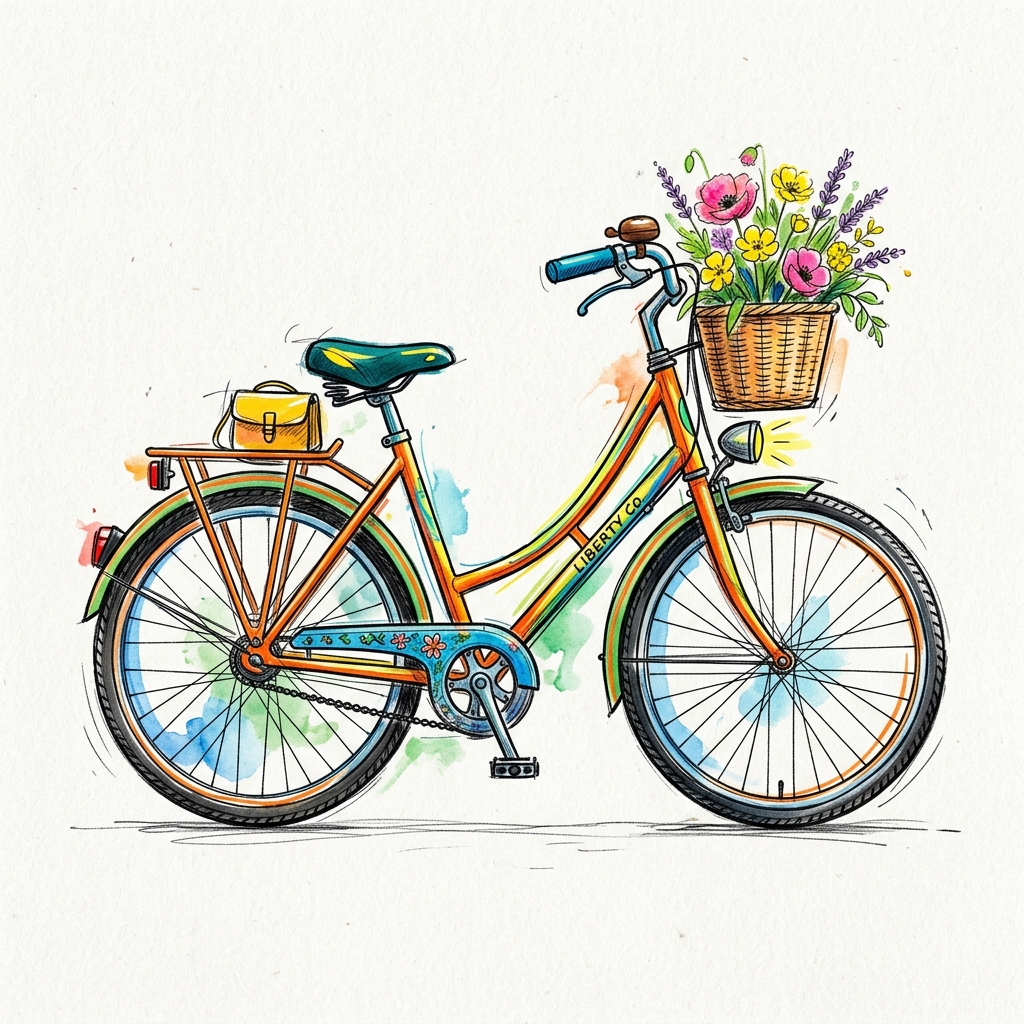
\includegraphics[width=0.9\linewidth]{vokab_300dpi/velo.png} \\
            \small\textit{De Vëlo (Le vélo / The bicycle)}
            \vspace{0.5cm}
        }}
    \end{minipage}
    \hfill
    \begin{minipage}[t]{0.48\textwidth}
        \centering
        \textbf{E Fliger}
        \vspace{0.5em}
        \framebox{\parbox{0.9\linewidth}{\centering
            \vspace{0.5cm}
            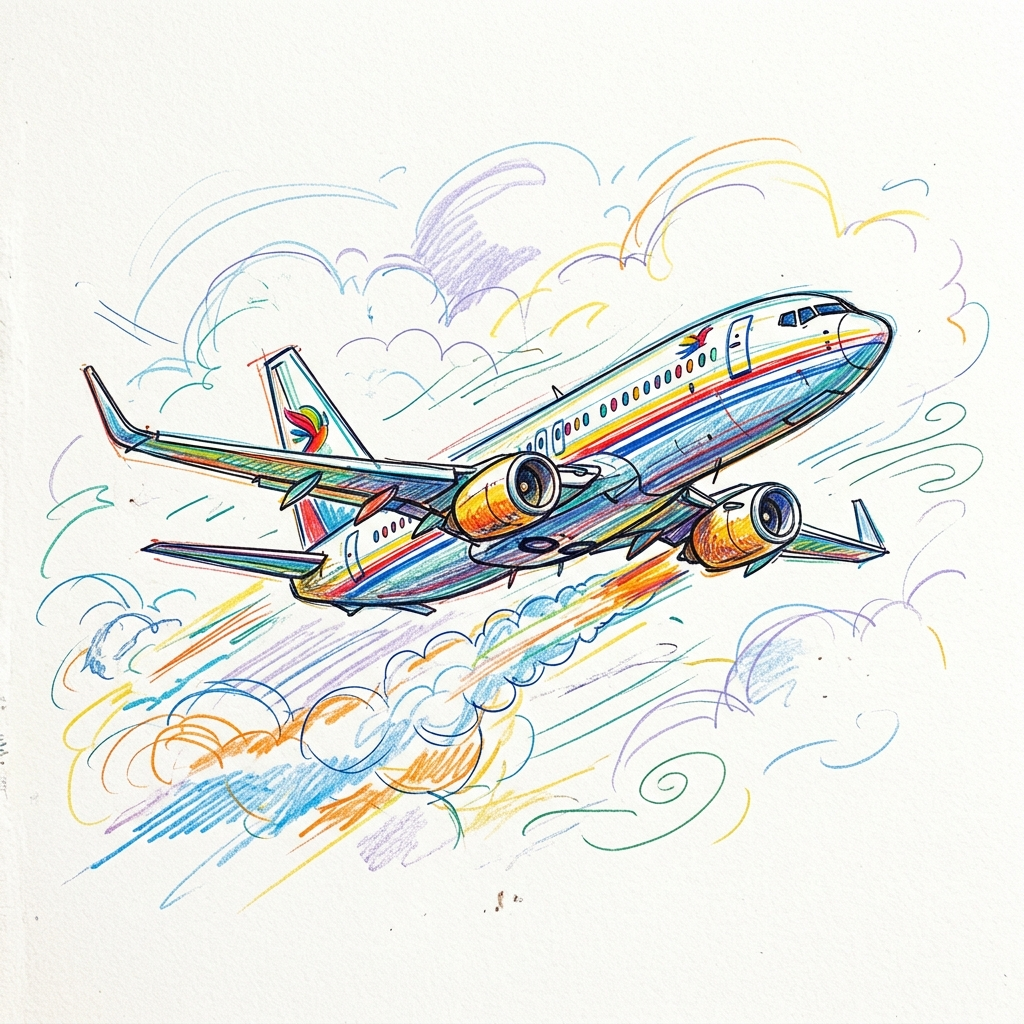
\includegraphics[width=0.9\linewidth]{vokab_300dpi/fliger.png} \\
            \small\textit{De Fliger (L'avion / The airplane)}
            \vspace{0.5cm}
        }}
    \end{minipage}
    
    \vspace{1.5em}
    
    \begin{minipage}[t]{0.48\textwidth}
        \centering
        \textbf{En Tram}
        \vspace{0.5em}
        \framebox{\parbox{0.9\linewidth}{\centering
            \vspace{0.5cm}
            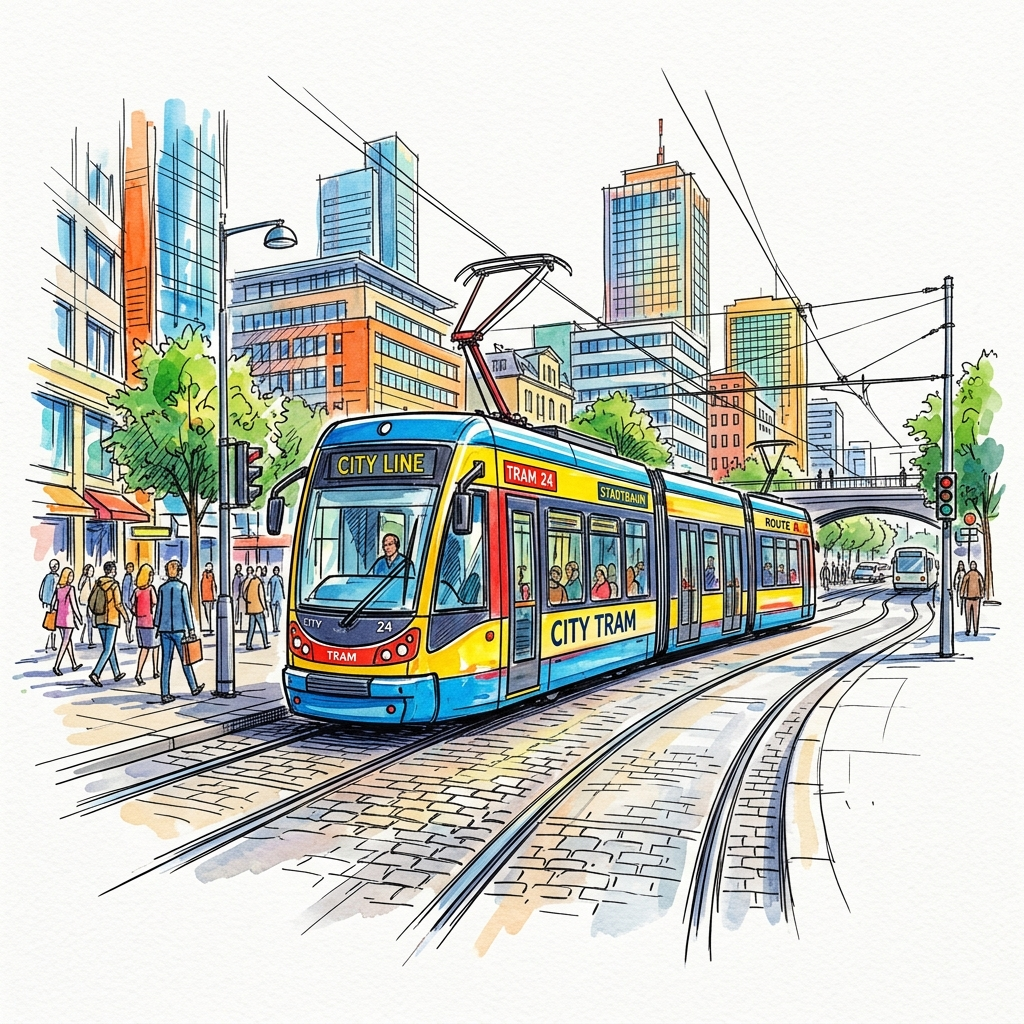
\includegraphics[width=0.9\linewidth]{vokab_300dpi/tram.png} \\
            \small\textit{Den Tram (Le tramway / The tram)}
            \vspace{0.5cm}
        }}
    \end{minipage}
    \hfill
    \begin{minipage}[t]{0.48\textwidth}
        \centering
        \textbf{Eng Harespel}
        \vspace{0.5em}
        \framebox{\parbox{0.9\linewidth}{\centering
            \vspace{0.5cm}
            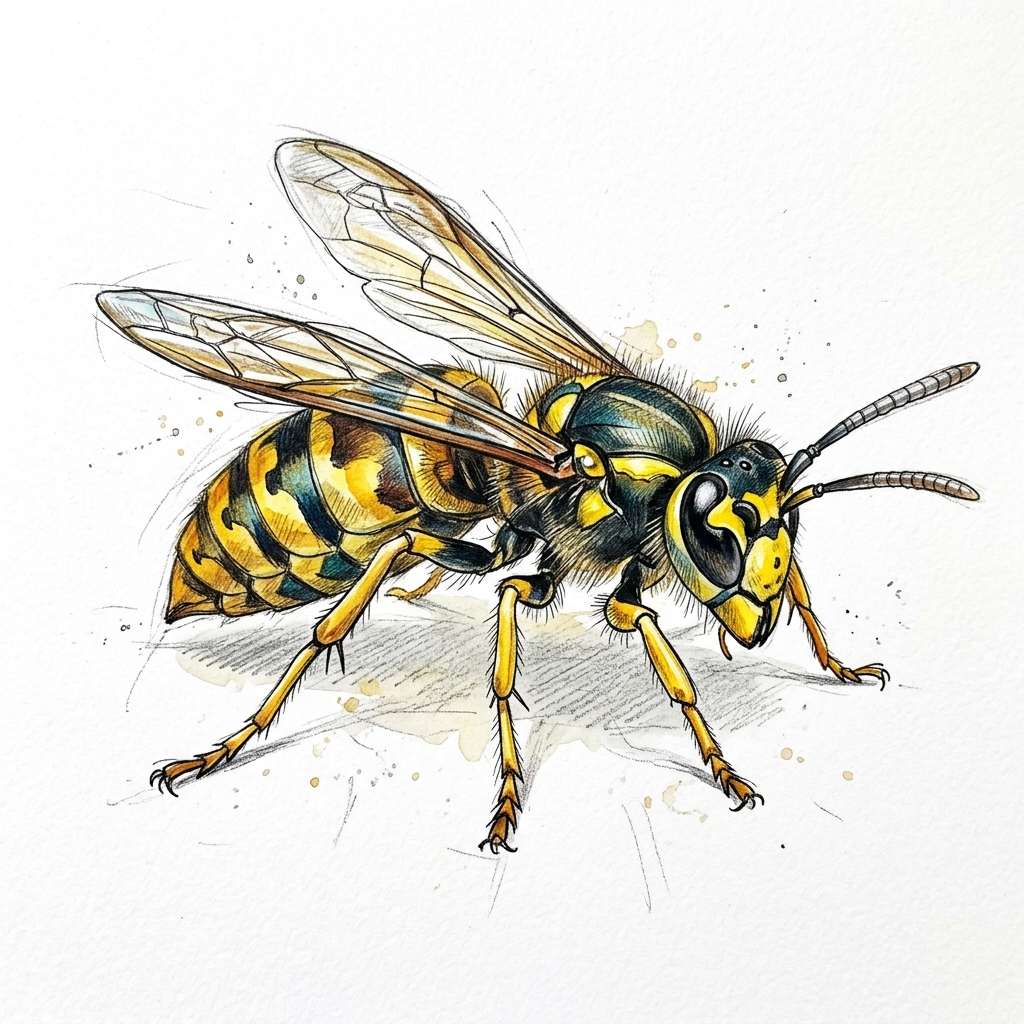
\includegraphics[width=0.9\linewidth]{vokab_300dpi/harespel.png} \\
            \small\textit{Eng Harespel (La guêpe / The wasp)}
            \vspace{0.5cm}
        }}
    \end{minipage}
    
    \vspace{1.5em}
    
    \begin{minipage}[t]{0.48\textwidth}
        \centering
        \textbf{E Containerschëff}
        \vspace{0.5em}
        \framebox{\parbox{0.9\linewidth}{\centering
            \vspace{0.5cm}
            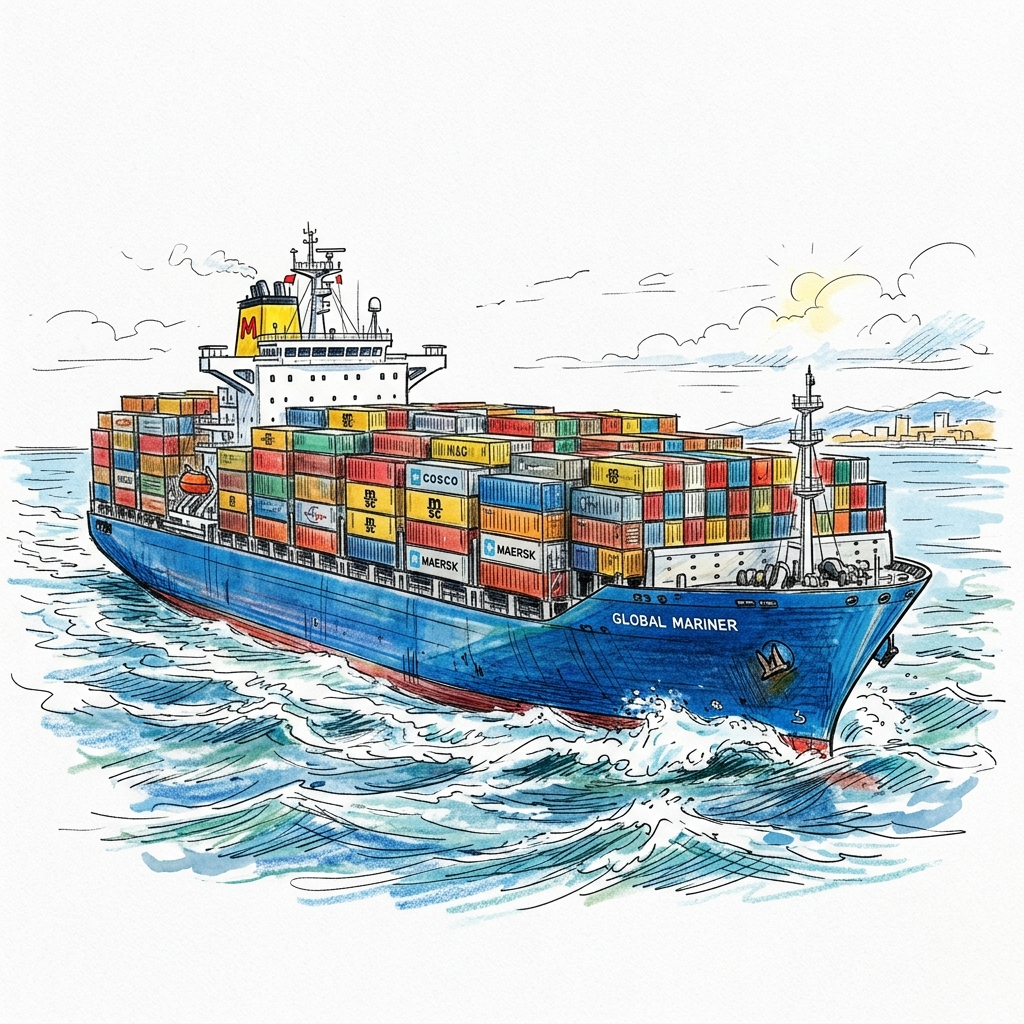
\includegraphics[width=0.9\linewidth]{vokab_300dpi/containerscheff.png} \\
            \small\textit{E Containerschëff (Le porte-conteneurs / The container ship)}
            \vspace{0.5cm}
        }}
    \end{minipage}
\end{center}
